\documentclass[11pt]{article}\usepackage[]{graphicx}\usepackage[]{color}
%% maxwidth is the original width if it is less than linewidth
%% otherwise use linewidth (to make sure the graphics do not exceed the margin)
\makeatletter
\def\maxwidth{ %
  \ifdim\Gin@nat@width>\linewidth
    \linewidth
  \else
    \Gin@nat@width
  \fi
}
\makeatother

\definecolor{fgcolor}{rgb}{0.345, 0.345, 0.345}
\newcommand{\hlnum}[1]{\textcolor[rgb]{0.686,0.059,0.569}{#1}}%
\newcommand{\hlstr}[1]{\textcolor[rgb]{0.192,0.494,0.8}{#1}}%
\newcommand{\hlcom}[1]{\textcolor[rgb]{0.678,0.584,0.686}{\textit{#1}}}%
\newcommand{\hlopt}[1]{\textcolor[rgb]{0,0,0}{#1}}%
\newcommand{\hlstd}[1]{\textcolor[rgb]{0.345,0.345,0.345}{#1}}%
\newcommand{\hlkwa}[1]{\textcolor[rgb]{0.161,0.373,0.58}{\textbf{#1}}}%
\newcommand{\hlkwb}[1]{\textcolor[rgb]{0.69,0.353,0.396}{#1}}%
\newcommand{\hlkwc}[1]{\textcolor[rgb]{0.333,0.667,0.333}{#1}}%
\newcommand{\hlkwd}[1]{\textcolor[rgb]{0.737,0.353,0.396}{\textbf{#1}}}%
\let\hlipl\hlkwb

\usepackage{framed}
\makeatletter
\newenvironment{kframe}{%
 \def\at@end@of@kframe{}%
 \ifinner\ifhmode%
  \def\at@end@of@kframe{\end{minipage}}%
  \begin{minipage}{\columnwidth}%
 \fi\fi%
 \def\FrameCommand##1{\hskip\@totalleftmargin \hskip-\fboxsep
 \colorbox{shadecolor}{##1}\hskip-\fboxsep
     % There is no \\@totalrightmargin, so:
     \hskip-\linewidth \hskip-\@totalleftmargin \hskip\columnwidth}%
 \MakeFramed {\advance\hsize-\width
   \@totalleftmargin\z@ \linewidth\hsize
   \@setminipage}}%
 {\par\unskip\endMakeFramed%
 \at@end@of@kframe}
\makeatother

\definecolor{shadecolor}{rgb}{.97, .97, .97}
\definecolor{messagecolor}{rgb}{0, 0, 0}
\definecolor{warningcolor}{rgb}{1, 0, 1}
\definecolor{errorcolor}{rgb}{1, 0, 0}
\newenvironment{knitrout}{}{} % an empty environment to be redefined in TeX

\usepackage{alltt}

%======================================================%
%-----------------------------------------------------------------------------------------------%
%****************************************************************************%
%++++++++++++++++++++++++++++++++++++++++++++++++++++++%
%~~~~~~~~~~~~~~~~~~~~~~~~~~~~~~~~~~~~~~~~~~~~~~~~~~~~~~%
%  My Packages and Commands %

%\usepackage{fullpage}
\usepackage{setspace}
\usepackage[left=1in,top=1in,right=1in]{geometry}
\pdfpagewidth 8.5in
\pdfpageheight 11in 
\setlength{\textheight}{9in}

%PLOTS
\usepackage{graphicx} %for importing graphics files
\usepackage{epstopdf}%for .eps files
\graphicspath{{figures/}}

% BIBLIOGRAPHY
\usepackage[authoryear]{natbib}
\bibpunct{(}{)}{;}{a}{}{,}
%\linespread{1.5}

\long\def\symbolfootnote[#1]#2{\begingroup
\def\thefootnote{\fnsymbol{footnote}}\footnote[#1]{#2}\endgroup}


\usepackage{amssymb, amsthm, amsmath, blindtext, enumitem}


%============================================
%============================================
%My New Commands
%============================================
\newcommand{\balpha}{\mbox{\boldmath $\alpha$} }
\newcommand{\bbeta}{\mbox{\boldmath $\beta$} }
\newcommand{\bdelta}{\mbox{\boldmath $\delta$} }
\newcommand{\bepsilon}{\mbox{\boldmath $\epsilon$} }
\newcommand{\bgamma}{\mbox{\boldmath $\gamma$} }
\newcommand{\blambda}{\mbox{\boldmath $\lambda$} }
\newcommand{\bmu}{\mbox{\boldmath $\mu$} }
\newcommand{\bnu}{\mbox{\boldmath $\nu$} }
\newcommand{\bomega}{\mbox{\boldmath $\omega$} }
\newcommand{\bphi}{\mbox{\boldmath $\phi$} }
\newcommand{\bpsi}{\mbox{\boldmath $\psi$} }
\newcommand{\brho}{\mbox{\boldmath $\rho$} }
\newcommand{\bsigma}{\mbox{\boldmath $\sigma$} }
\newcommand{\btau}{\mbox{\boldmath $\tau$} }
\newcommand{\btheta}{\mbox{\boldmath $\theta$} }
\newcommand{\bupsilon}{\mbox{\boldmath $\upsilon$} }
\newcommand{\bxi}{\mbox{\boldmath $\xi$} }
\newcommand{\bzeta}{\mbox{\boldmath $\zeta$} }
\newcommand{\bDelta}{\mbox{\boldmath $\Delta$} }
\newcommand{\bGamma}{\mbox{\boldmath $\Gamma$} }
\newcommand{\bLambda}{\mbox{\boldmath $\Lambda$} }
\newcommand{\bPhi}{\mbox{\boldmath $\Phi$} }
\newcommand{\bSigma}{\mbox{\boldmath $\Sigma$} }
\newcommand{\bTheta}{\mbox{\boldmath $\Theta$} }

\newcommand{\bfa}{\mbox{\bf a} }
\newcommand{\bfb}{\mbox{\bf b} }
\newcommand{\bfc}{\mbox{\bf c} }
\newcommand{\bfd}{\mbox{\bf d} }
\newcommand{\bfe}{\mbox{\bf e} }
\newcommand{\bff}{\mbox{\bf f} }
\newcommand{\bfg}{\mbox{\bf g} }
\newcommand{\bfh}{\mbox{\bf h} }
\newcommand{\bfi}{\mbox{\bf i} }
\newcommand{\bfj}{\mbox{\bf j} }
\newcommand{\bfk}{\mbox{\bf k} }
\newcommand{\bfl}{\mbox{\bf l} }
\newcommand{\bfm}{\mbox{\bf m} }
\newcommand{\bfn}{\mbox{\bf n} }
\newcommand{\bfo}{\mbox{\bf o} }
\newcommand{\bfp}{\mbox{\bf p} }
\newcommand{\bfq}{\mbox{\bf q} }
\newcommand{\bfr}{\mbox{\bf r} }
\newcommand{\bfs}{\mbox{\bf s} }
\newcommand{\bft}{\mbox{\bf t} }
\newcommand{\bfu}{\mbox{\bf u} }
\newcommand{\bfv}{\mbox{\bf v} }
\newcommand{\bfw}{\mbox{\bf w} }
\newcommand{\bfx}{\mbox{\bf x} }
\newcommand{\bfy}{\mbox{\bf y} }
\newcommand{\bfz}{\mbox{\bf z} }
\newcommand{\bfA}{\mbox{\bf A} }
\newcommand{\bfB}{\mbox{\bf B} }
\newcommand{\bfC}{\mbox{\bf C} }
\newcommand{\bfD}{\mbox{\bf D} }
\newcommand{\bfE}{\mbox{\bf E} }
\newcommand{\bfF}{\mbox{\bf F} }
\newcommand{\bfG}{\mbox{\bf G} }
\newcommand{\bfH}{\mbox{\bf H} }
\newcommand{\bfI}{\mbox{\bf I} }
\newcommand{\bfJ}{\mbox{\bf J} }
\newcommand{\bfK}{\mbox{\bf K} }
\newcommand{\bfL}{\mbox{\bf L} }
\newcommand{\bfM}{\mbox{\bf M} }
\newcommand{\bfN}{\mbox{\bf N} }
\newcommand{\bfO}{\mbox{\bf O} }
\newcommand{\bfP}{\mbox{\bf P} }
\newcommand{\bfQ}{\mbox{\bf Q} }
\newcommand{\bfR}{\mbox{\bf R} }
\newcommand{\bfS}{\mbox{\bf S} }
\newcommand{\bfT}{\mbox{\bf T} }
\newcommand{\bfU}{\mbox{\bf U} }
\newcommand{\bfV}{\mbox{\bf V} }
\newcommand{\bfW}{\mbox{\bf W} }
\newcommand{\bfX}{\mbox{\bf X} }
\newcommand{\bfY}{\mbox{\bf Y} }
\newcommand{\bfZ}{\mbox{\bf Z} }

\newcommand{\calA}{{\cal A}}
\newcommand{\calB}{{\cal B}}
\newcommand{\calC}{{\cal C}}
\newcommand{\calD}{{\cal D}}
\newcommand{\calE}{{\cal E}}
\newcommand{\calF}{{\cal F}}
\newcommand{\calG}{{\cal G}}
\newcommand{\calH}{{\cal H}}
\newcommand{\calI}{{\cal I}}
\newcommand{\calJ}{{\cal J}}
\newcommand{\calK}{{\cal K}}
\newcommand{\calL}{{\cal L}}
\newcommand{\calM}{{\cal M}}
\newcommand{\calN}{{\cal N}}
\newcommand{\calO}{{\cal O}}
\newcommand{\calP}{{\cal P}}
\newcommand{\calQ}{{\cal Q}}
\newcommand{\calR}{{\cal R}}
\newcommand{\calS}{{\cal S}}
\newcommand{\calT}{{\cal T}}
\newcommand{\calU}{{\cal U}}
\newcommand{\calV}{{\cal V}}
\newcommand{\calW}{{\cal W}}
\newcommand{\calX}{{\cal X}}
\newcommand{\calY}{{\cal Y}}
\newcommand{\calZ}{{\cal Z}}

\renewcommand{\Hat}{\widehat}
\renewcommand{\Bar}{\overline}
\renewcommand{\Tilde}{\widetilde}

\newcommand{\iid}{\stackrel{iid}{\sim}}
\newcommand{\indep}{\overset{ind}{\sim}}
%\newcommand{\argmax}{{\mathop{\rm arg\, max}}}
%\newcommand{\argmin}{{\mathop{\rm arg\, min}}}
\newcommand{\Frechet}{ \mbox{Fr$\acute{\mbox{e}}$chet} }
\newcommand{\Matern}{ \mbox{Mat$\acute{\mbox{e}}$rn} }

\providecommand{\argmin}[1]{\underset{{#1}}{\rm \ argmin}} 
\providecommand{\argmax}[1]{\underset{{#1}}{\rm \ argmax}} 

\newcommand{\seteq}{\stackrel{set}{\ =\ }}


\newcommand{\bfig}{\begin{figure}}
\newcommand{\efig}{\end{figure}}
\newcommand{\beqx}{\begin{equation*}}
\newcommand{\eeqx}{\end{equation*}}
\newcommand{\beq}{\begin{equation}}
\newcommand{\eeq}{\end{equation}}
\newcommand{\beqa}{\begin{eqnarray}}
\newcommand{\eeqa}{\end{eqnarray}}
\newcommand{\beqax}{\begin{eqnarray*}}
\newcommand{\eeqax}{\end{eqnarray*}}
\newcommand{\beqn}{\begin{dmath}}
\newcommand{\eeqn}{\end{dmath}}
\newcommand{\beqnx}{\begin{dmath*}}
\newcommand{\eeqnx}{\end{dmath*}}

\let\originalleft\left
\let\originalright\right
\renewcommand{\left}{\mathopen{}\mathclose\bgroup\originalleft}
\renewcommand{\right}{\aftergroup\egroup\originalright}

\providecommand{\itbf}[1]{\textit{\textbf{#1}}} 
\providecommand{\abs}[1]{\left\lvert#1\right\rvert} 
\providecommand{\norm}[1]{\left\lVert#1\right\rVert}

\newcommand{\cond}{\,\left\vert\vphantom{}\right.}
\newcommand{\Cond}{\,\Big\vert\vphantom{}\Big.}
\newcommand{\COND}{\,\Bigg\vert\vphantom{}\Bigg.}

\providecommand{\paren}[1]{\left(#1\right)} 
\providecommand{\Paren}[1]{\Big(#1\Big)}
\providecommand{\PAREN}[1]{\bigg(#1\bigg)} 
\providecommand{\bracket}[1]{\left[ #1 \right]} 
\providecommand{\Bracket}[1]{\Big[ #1 \Big]} 
\providecommand{\BRACKET}[1]{\bigg[ #1 \bigg]} 
\providecommand{\curlybrace}[1]{\left\{ #1 \right\}} 
\providecommand{\Curlybrace}[1]{\Big\{ #1 \Big\}} 
\providecommand{\CURLYBRACE}[1]{\bigg\{ #1 \bigg\}} 

\newcommand{\Bern}{\mbox{{\sf Bern}}}
\newcommand{\Bernoulli}{\mbox{{\sf Bernoulli}}}
\newcommand{\Beta}{\mbox{{\sf Beta}}}
\newcommand{\Bin}{\mbox{{\sf Bin}}}
\newcommand{\Binomial}{\mbox{{\sf Binomial}}}
\newcommand{\DE}{\mbox{{\sf DE}}}
\newcommand{\Exponential}{\mbox{{\sf Exponential}}}
\newcommand{\F}{\mbox{{\sf F}}}
\newcommand{\Gam}{\mbox{{\sf Gamma}}}
\newcommand{\GP}{\mbox{{\sf GP}}}
\newcommand{\GPD}{\mbox{{\sf GPD}}}
\newcommand{\Geom}{\mbox{{\sf Geom}}}
\newcommand{\Geometric}{\mbox{{\sf Geometric}}}
\newcommand{\HyperGeom}{\mbox{{\sf HyperGeom}}}
\newcommand{\HyperGeometric}{\mbox{{\sf HyperGeometric}}}
\newcommand{\InverseGam}{\mbox{{\sf InverseGamma}}}
\newcommand{\InvWish}{\mbox{{\sf InvWish}}}
\newcommand{\MVN}{\mbox{{\sf MVN}}}
\newcommand{\NB}{\mbox{{\sf NB}}}
\newcommand{\NegBin}{\mbox{{\sf NegBin}}}
\newcommand{\NegativeBinomial}{\mbox{{\sf NegativeBinomial}}}
\newcommand{\Normal}{\mbox{{\sf Normal}}}
\newcommand{\Pois}{\mbox{{\sf Pois}}}
\newcommand{\Poisson}{\mbox{{\sf Poisson}}}
\newcommand{\Unif}{\mbox{{\sf Unif}}}
\newcommand{\Uniform}{\mbox{{\sf Uniform}}}
\newcommand{\Weibull}{\mbox{{\sf Weibull}}}

\renewcommand{\P}{{\sf P}}
\newcommand{\Prob}{{\sf Prob}}
\newcommand{\median}{{\mathop{\rm median}}}
\newcommand{\E}{\mathsf{E}}
\newcommand{\V}{\mathsf{V}}
\newcommand{\VAR}{\mathsf{VAR}}
\newcommand{\COV}{\mathsf{COV}}

\newcommand{\Ho}{{\calH_0}}
\newcommand{\Hoc}{{\calH_0\colon}}
\newcommand{\Hone}{{\calH_1}}
\newcommand{\Honec}{{\calH_1\colon}}
\newcommand{\Ha}{{\calH_a}}
\newcommand{\Hac}{{\calH_a\colon}}
\newcommand{\HA}{{\calH_A}}
\newcommand{\HAc}{{\calH_A\colon}}


\newcommand{\Ind}{\mathds{1}}
\newcommand{\zerovect}{\mbox{\bf 0}}
\newcommand{\onesvect}{\mbox{\bf 1}}
\providecommand{\real}[1]{\mathbb{#1}}
\newcommand{\Real}{\mathbb{R}}
\newcommand{\ppd}{\mathcal{P}}
\DeclareMathOperator{\logit}{logit}
\DeclareMathOperator{\expit}{expit}
\DeclareMathOperator{\dint}{\displaystyle\int}
\DeclareMathOperator{\dsum}{\displaystyle\sum}

%============================================
%My New Commands
%============================================
%============================================




\newcommand{\bitemize}{\begin{itemize}\setlength{\itemsep}{1pt}\setlength{\parskip}{1pt}}
\newcommand{\eitemize}{\end{itemize}}
\newcommand{\benum}{\begin{enumerate}\setlength{\itemsep}{1pt}\setlength{\parskip}{1pt}}
\newcommand{\eenum}{\end{enumerate}}

\usepackage{fancyhdr}
\pagestyle{fancy}

%\lhead{\footnotesize \parbox{11cm}{Custom left-head-note} }
\cfoot{}
\lfoot{\footnotesize \parbox{11cm}{}}
\rfoot{\footnotesize Page \thepage\ }
%\rfoot{\footnotesize Page \thepage\ of \pageref{LastPage}}
%\renewcommand\headheight{24pt}
\renewcommand\footrulewidth{0.4pt}


\usepackage[colorlinks=false,
          %  pdfborder={0 0 0},
            ]{hyperref}


%  My Packages and Commands %
%======================================================%
%-----------------------------------------------------------------------------------------------%
%****************************************************************************%
%++++++++++++++++++++++++++++++++++++++++++++++++++++++%
%~~~~~~~~~~~~~~~~~~~~~~~~~~~~~~~~~~~~~~~~~~~~~~~~~~~~~~%
%______________________________________________________%
\IfFileExists{upquote.sty}{\usepackage{upquote}}{}
\begin{document}%\linenumbers





\title{\bf Bayesian Estimation of Modified ETAS Model for Invasive Species}
\author{Binhui Deng \and Earvin Balderama}
%\date{}
\maketitle


%============================================
%============================================
\abstract{

The Epidemic-Type Aftershock Sequence (ETAS) model, a \cite{Hawkes71} self-exciting point process model, is commonly used for characterizing earthquake and aftershock activity.
Red banana trees, an invasive plant in Costa Rican rainforest, have been being observed for recent few years. Adjusted ETAS model was applied onto the study of red banana tree to characterize it's spatial-temporal spreading patterns. 
This project proposed Bayesian Markov Chain Monte Carlo method to estimate unknown parameters in the adjusted ETAS model.\\

{\bf Keywords}: epidemic type aftershock sequence models, bayesian, MCMC, invasive species
%============================================
%============================================


%============================================
\section{Introduction}
%============================================

Invasive species is a subset of introduced species. It would be defined as an invasive species if a species is artificially introduced into a region that it has not previously existed and has the capacity to grow into a certain amount in the absence of human intervention, then threaten local biodiversity and become a local hazard.

Invasive alien species of plants can also destroy the habitat of native species and disturb the natural evolution that takes place in the environment in which they spread. Many invasive plant species have been studied in the past \citep{Higgins96,Delisle03}. Too many of these studies simply report statistics based on amount of land consumed over some period of time. Of these, most do not report precise locations where these plants are spreading. There are a couple of reasons why this is the case: 1) Computational methods are either too simple or too difficult, and 2) Data on the invasive species do not contain exact locations of each individual plant. Even when trying to analyze the current and future locations of invasive plants, the models do not come from point process methodology. Instead, studies often use grid-based methods, where the surface of study is divided into an array of pixels on a grid.

The natural process by which plants can spread its seeds initiates the conversation of statistically analyzing the spatial and temporal spread of invasive plants using the theory of point processes. According to the former research done by Dr. Earvin Balderama, the estimates obtained by Newton-Rhapson numerical optimization were $\boldsymbol{\hat\theta} = \{\hat\alpha = 0.0760, \hat\beta = 0.0292, \hat p = 0.5770\}$, with corresponding asymptotic standard errors 0.0045, 0.0022 and 0.0190, respectively. 

The Bayesian MCMC algorithm was of interest to retrospectively examine if more accurate estimates could be obtained and if the estimates are robust.
%============================================
\section{Data}
%============================================



The data studied in \cite{Balderama12} contained the precise longitude and latitude coordinates, captured by Global Position System (GPS), of red banana trees that has spread through a significant part of a rainforest in Costa Rica. In addition to location, the height (in cm) and other variables of each tree was also measured. With the information available, it was then easy to map the trees as a spatial point process. Note that there is no need to use the height variable to create a {\it marked} spatial point process, because these marks will offer no direct knowledge on how these plants are spreading. Instead, because of the partial dependency of age as it relates to the height of a tree, birth times of the red banana trees were estimated, allowing for a temporal analysis of spread.


We use the red banana data from \cite{Balderama12}. Heights (in cm) of 1008 red banana plants were observed and longitude and latitude coordinates were recorded by satellite. The heights of 318 select plants were measured weekly over a span of one year. To establish a time component, estimates of the growth rate was used to estimate any individual plant's age, and hence origin times. In the end, 788 plants had complete location and origin times data, and were used for the subsequent analyses.

\bfig\centering
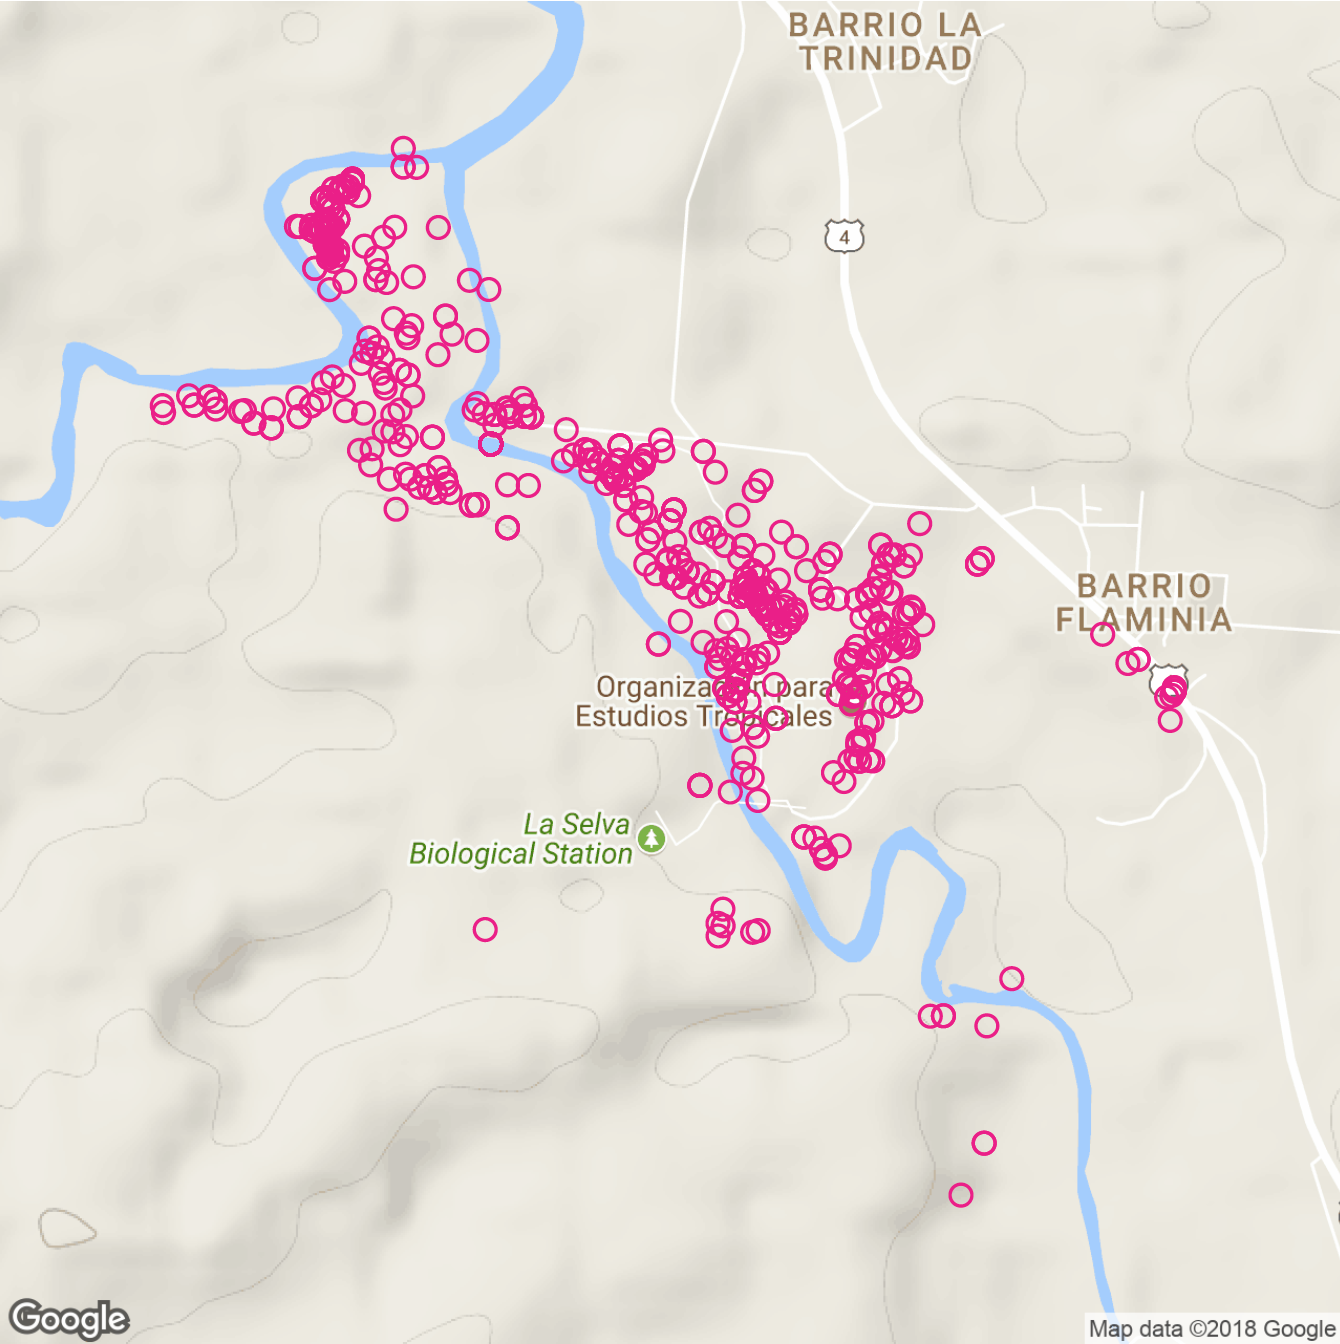
\includegraphics[width=5cm]{figures/redbanana.png}
\caption{}
\label{Map1}
\efig

%============================================
\section{Methods}
%============================================

Ogata's epidemic-type aftershock sequence models \citep{Ogata88,Ogata98} is one of the most popular models of earthquake occurrences. The ETAS model is so aptly names because of the epidemic nature of how events are created; Earthquakes causes aftershocks, which in turn causes more aftershocks, and so on. It characterizes a sequence of earthquakes and aftershocks over time or over space and time via a conditional intensity, which represents the infinitesimal probability of an event occurrence at a single point in $\real{R}^d$ given the past history of the process. This particular characterization of a sequence of earthquakes and aftershocks is a specific case of the linear, self-exciting Hawkes' point process \citep{Hawkes71}, which is specified by the conditional intensity
\begin{equation}\label{hawkes}
\lambda(t, Q \cond H_t) = \mu(t,Q) + \sum_{t_i < t} g(t,Q; t_i, Q_i),
\end{equation}
where $Q$ is additional information that may include a spatial component $(x,y)$ and/or a mark or magnitude $M$, $H_t$ is the history of the process up to time $t$, $\mu(\cdot)$ is the mean rate of a Poisson-distributed background process that may depend on time, space and magnitude, and $g(\cdot)$ is the ``triggering function" which contributes the individual intensities of each point $\{i: t_i < t\}$ as a summation to the total conditional intensity $\lambda(\cdot)$ at time $t$. Thus, every past event has an additive (linear) influence on the present conditional intensity of the system.

A modified version of this Hawkes/ETAS model was empirically fitted to the red banana data \citep{Balderama12}. First, the spatially inhomogeneous background density $\hat\mu(x,y)$ was estimated by a two-dimensional Guassian kernel smoother over the complete data. Next, a close examination of interevent distances and times between pairs of plants constituted an exponential decay in both time lag and squared distance. The triggering density function is then given by
\begin{equation}\label{gredbanana}
g(t,x,y) = \dfrac{\alpha \beta}{\pi} \cdot e^{-\alpha t - \beta(x^2+y^2)},
\end{equation}
where $\frac{\alpha\beta}{\pi}$ is a normalizing constant so that $g$ integrates to one. The conditional intensity was then specified as 
\begin{equation}\label{etasplants}
\lambda(t,x,y | H_t) = (1-p)\mu(x,y) + \dfrac{p \alpha \beta}{\pi} \sum_{\{i:t_i < t\}} e^{-\alpha (t-t_i) - \beta\{(x-x_i)^2+(y-y_i)^2\}}
\end{equation}
where $p$ is introduced to specify the proportion of events that were triggered, leading to a simultaneous estimation of the parameter vector $\boldsymbol{\theta} = \{\alpha, \beta, p\}$ by utilizing Bayesian Markov Chain Monte Carlo algorithm. Both $\alpha$ and $\beta$ are parameters should be greater than zero, the prior distributions for them were then set to be Gamma($\alpha_a$, $\beta_a$) and Gamma($\alpha_b$, $\beta_b$), respectively, where $\alpha_a$ and $\alpha_b$ were set to be 1, and $\beta_a$ and $\beta_b$ had uninformative hyper prior distributions, Gamma($\alpha_{hyper}$, $\beta_{hyper}$), where $\alpha_{hyper}$=$\beta_{hyper}$=0.5. For parameter $p$, which indicates an unknown proportion, should range between 0 and 1, so Uniform(0,1) was set as the prior distribution. The log-likelihood was then specified as
\begin{equation}
logL = \sum_{i=1}^{n} log\lambda(t_i,x_i,y_i) - \iint_A \int_{0}^{\infty}\lambda(t,x,y)dtdxdy.
\end{equation}

The symmetric proposal distributions for $\alpha$ and $\beta$ were set to be Normal($\alpha^{(t-1)}$,0.1) and Normal($\beta^{(t-1)}$,0.1) respectively, and the asymmetric proposal distribution for paramater $p$ is Beta($p^{(t-1)}$,$1-p^{(t-1)}$), which has mean of $p^{(t-1)}$. The symbols $\alpha^{(t-1)}$, $\beta^{(t-1)}$ and $p^{(t-1)}$ represent the current values of parameters. 

Because hyper prior distributions are conjugate priors, candidates of $\beta_a$ and $\beta_b$ were directly updated from their posterior distributions, $Gamma(\alpha_{hyper}+n\alpha_a, \beta_{hyper}+\textstyle \sum _{i=1}^n \alpha )$ and $Gamma(\alpha_{hyper}+n\alpha_b, \beta_{hyper}+\textstyle \sum _{i=1}^n \beta )$. Potential candidates of parameters would be drawn from proposal distributions and be updated by using Metropolis-Hastings ratio technique, which is specified as
\begin{equation}
R = \frac{p(\theta^{(c)}|y)}{p(\theta^{(t-1)}|y)},
\end{equation}
where $\theta^{(c)}$ represents the candidate parameter and $\theta^{(t-1)}$ indicates the current parameter. The parameter $\theta^{(t)}$ would be updated to $\theta^{(c)}$ at certain probability or remain as $\theta^{(t-1)}$.

After the Bayesian MCMC algorithm, 50,000 potential candidates for each parameter were recorded. Thining technique was applied, which discarded all but $10^{th}$ observations to get rid of autocorrelation to guarantee the independecy of samples, and 5,000 observations were left. Burning technique was then utilized, which threw away first 2,500 observations to minimize the effect of initial values on the posterior inference.
Tuning technique was applied as well, which controlled the acceptence rate in a desired range, 25\% to 60\%. Bayesian inferences were then conducted based on the final 2,500 observations.  







%========================
\section{Results}
%========================

The trace plot and posterior histogram for each parameter are shown in Figure~\ref{Post1}. 

\bfig\centering
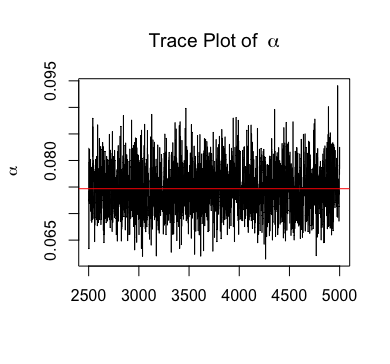
\includegraphics[width=4cm]{figures/gamma0505/a_trace.png}
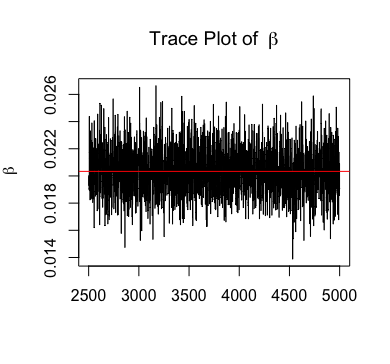
\includegraphics[width=4cm]{figures/gamma0505/b_trace.png}
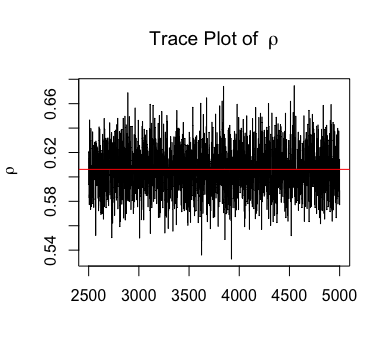
\includegraphics[width=4cm]{figures/gamma0505/p_trace.png}\\
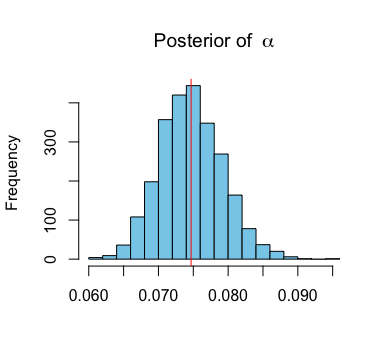
\includegraphics[width=4cm]{figures/gamma0505/a_hist.png}
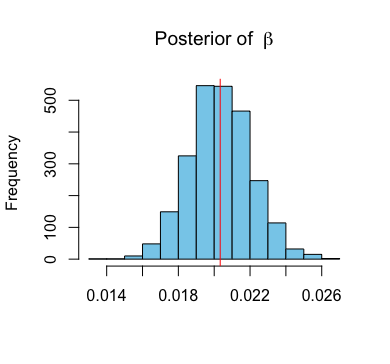
\includegraphics[width=4cm]{figures/gamma0505/b_hist.png}
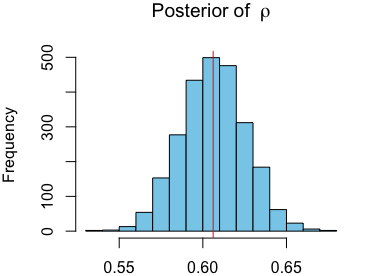
\includegraphics[width=4cm]{figures/gamma0505/p_hist.png}
\caption{}
\label{Post1}
\efig

The estimates obtained by Bayesian MCMC algorithm were $\boldsymbol{\hat\theta} = \{\hat\alpha = 0.0747, \hat\beta = 0.0203, \hat p = 0.6062\}$, with corresponding posterior standard deviations 0.0045, 0.0017 and 0.01941, respectively. These estimates are used to explain the decay rates of triggering events, where $\hat\alpha = 0.0747$ represents the intensity of trggering events decays at a a rate of $1-e^{-0.0747}=7.198\%$ for every week that passes, $\hat\beta = 0.0203$ suggests that the intensity of trggering events decays at a a rate of $1-e^{-0.0203}=2.1\%$ for every squared distance (in meters) away and $\hat\rho = 0.6062$ indicates that 60.62\% of events were triggered by observed plants and 39.38\% is due to the background rate (i.e., unobserved plants or other unknown sources). It is worth noting that this space-time modification does not contain magnitude information, as is the case for earthquakes, and that the dependence on time $t$ is removed from the estimation of the background rate, as is also the case with Ogata's ETAS models.

The estimates from Bayesian MCMC are very close to the ones from Newton-Rhapson numerical optimization, and the posterior standard deviations are smaller than asymptotic standard errors for most of time.

Figure~\ref{Sims1} show three simulations of the spreading pattern of red banana plants by using the modified ETAS model with Bayesian estimates.

\bfig\centering
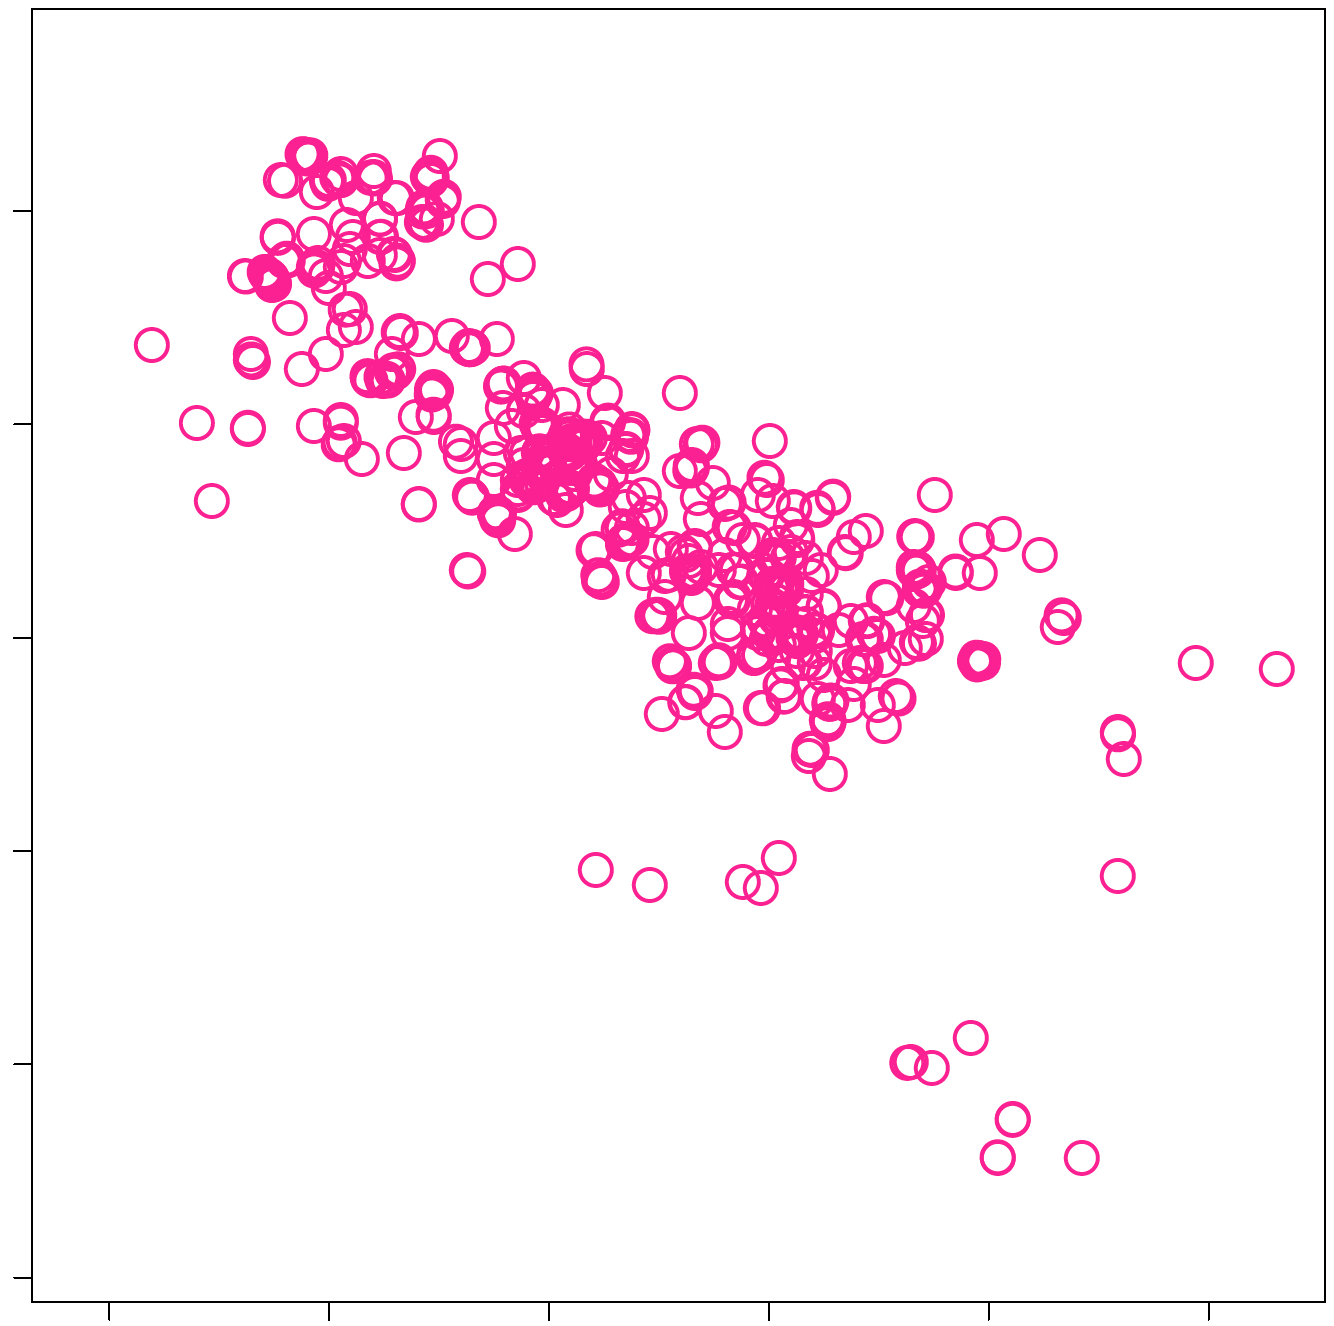
\includegraphics[width=4cm]{figures/simulation1.png}
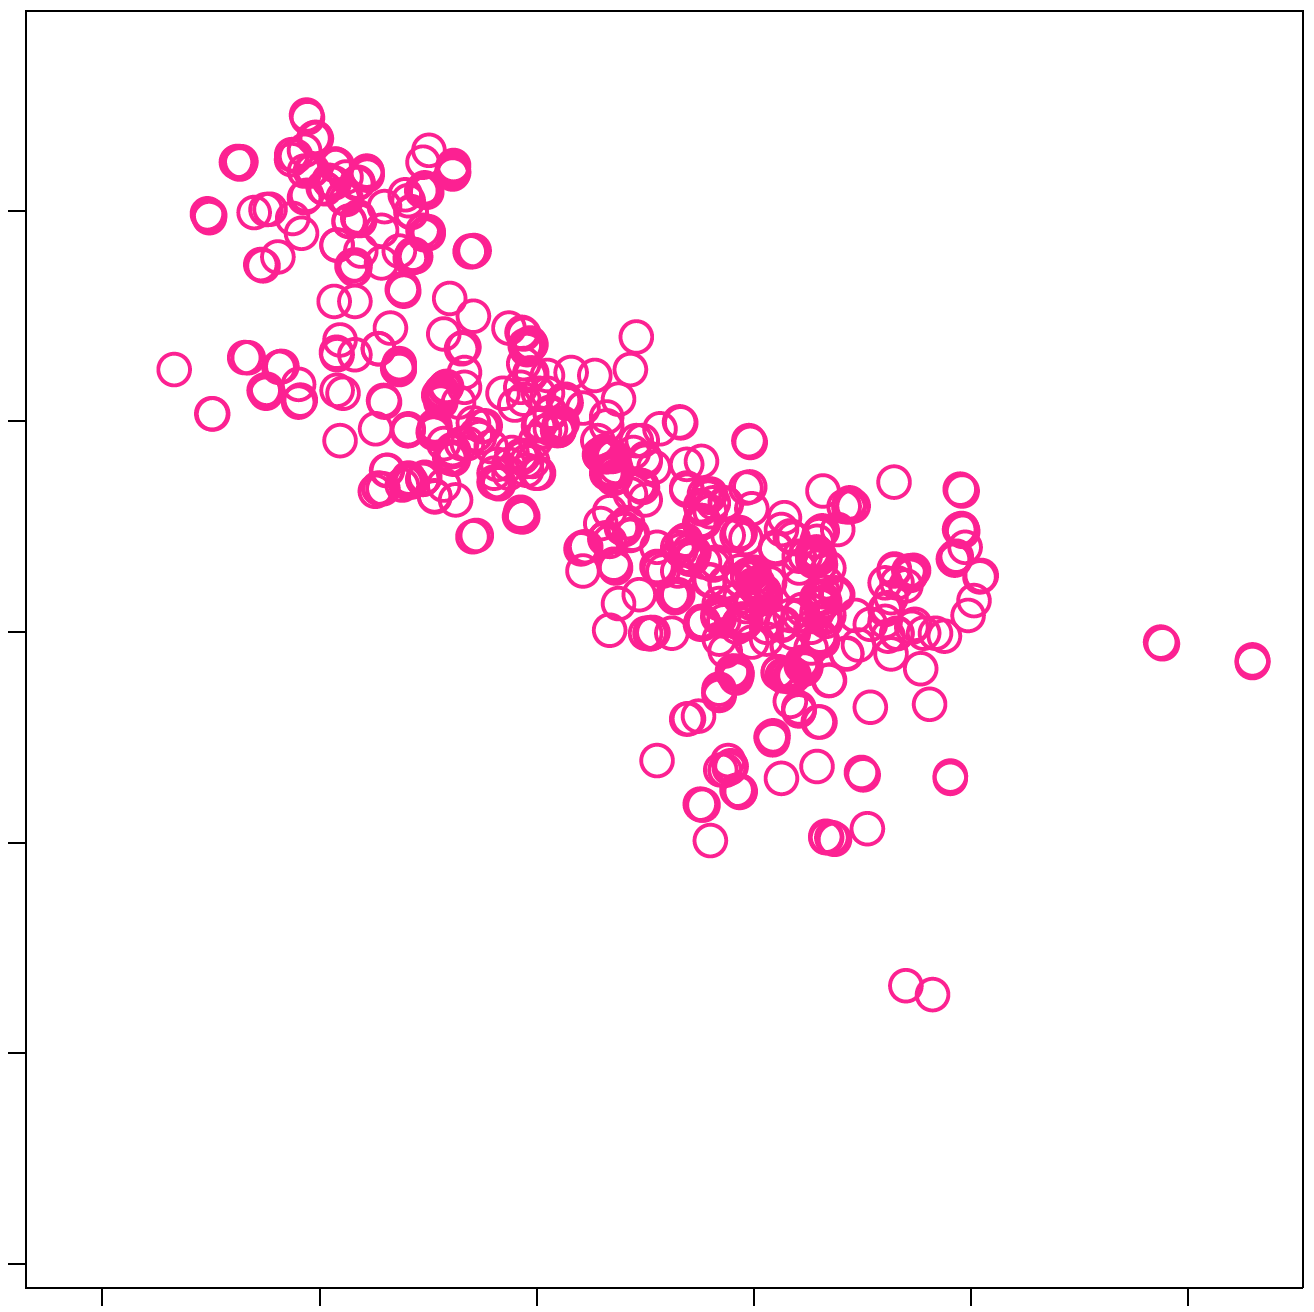
\includegraphics[width=4cm]{figures/simulation2.png}
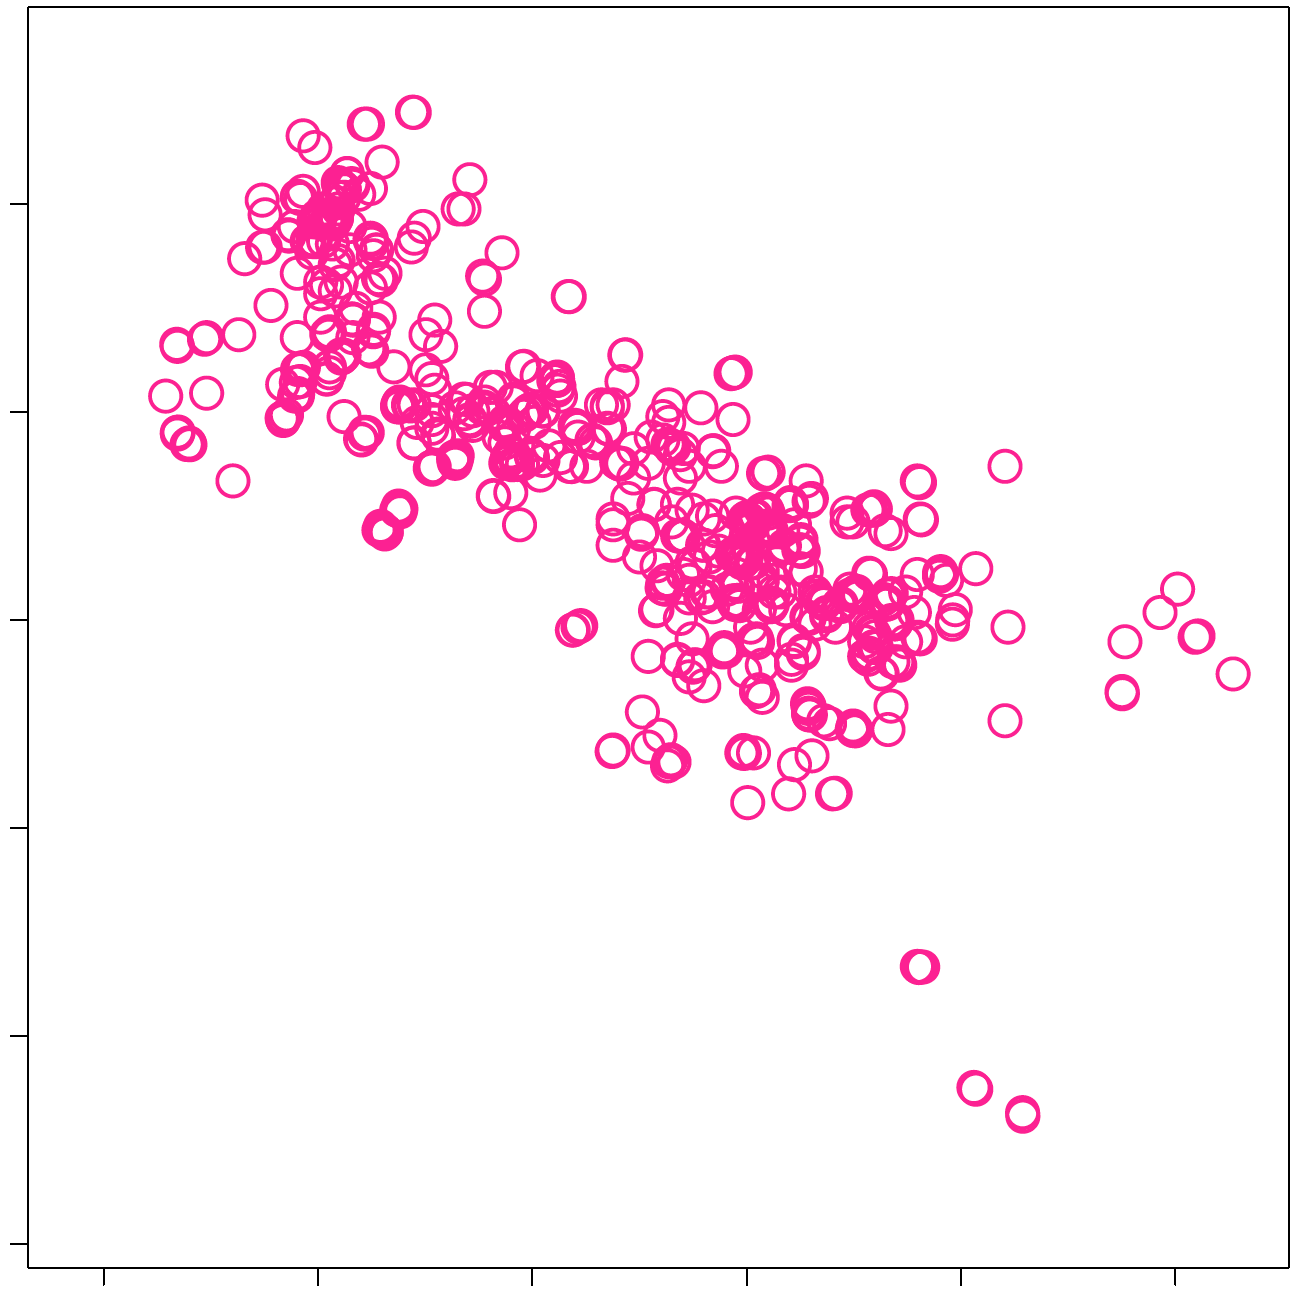
\includegraphics[width=4cm]{figures/simulation3.png}
\caption{}
\label{Sims1}
\efig

 Furthermore, this model was empirically fitted using the red banana data, and is therefore another case of a self-excited Hawkes' point process. A different species of plants may require not only different estimates of the parameters, but possibly a different set of parameters altogether, depending on the spatial and temporal distributions of interevent distances and times. However, it was the first attempt at using ETAS models to characterize the branching structure of invasive plant species.

\bibliographystyle{asa}
\bibliography{earvin2}



\end{document}
